\subsubsection{Primer 2 - Potapanje brodica}

\large{1. Opis zadatka}
\normalsize

Napraviti Client-Server aplikaciju koja će komunicirati na TCP portu X (gde je $X = broj\ indeksa / 24 + 2000)$ i omogućavati klijentima da igraju igru potapanja brodova.

\large{2. Opis igre}
\normalsize

Ovo je popularna i zabavna igra za dva igrača. Cilj igre je potopiti sve brodove protivničke mornarice. Ova igra se pojavljivala na nekolicini takmičenja, uključujući Svetsko takmičenje u slagalicama, i magazinima o slagalicama, kao što je magazin Games.

Igra se na tabli veličine $9\times9$, vrste su označene slovima abecede A-J, dok su kolone označene brojevima 1-9. Pre nego što počne igra, svaki igrač tajno postavi brodove nasvojoj glavnoj tabli. Svaki igrač ima 5 tipova brodova koje raspoređuje na svojoj 9x9 tabli.Veličine brodova su: $1\times5$, $1\times4$, $1\times3$, $1\times2$, $1\times1$. Igrači imaju po dva broda dimenzija $1\times1$ i $1\times2$ i po jedan svih ostalih dimenzija, koje postavljaju na tablu u bilo kojoj orijentaciji ($1\times5$ ili $5\times1$). Sva polja koja zauzima brod moraju biti poravnata duž jedne linije, orijentisana horizontalno ili vertikalno. Brodovi se mogu dodirivati, ali se ne mogu preklapati, tj. na jednom polju se može nalaziti samo jedan brod, kao što je prikazano na slici. Svaki igračdobija isti broj i vrstu brodova.

\begin{figure}[H]
    \centering
    
\includegraphics[width=0.5\textwidth]{Slike/PTP/Dozvoljene pozicije.png}
    \caption*{Primer dozvoljene postavke brodova}
    \label{fig:dozvoljene_postavke}
\end{figure}

\newpage
\large{3. Specifikacija zadatka}
\normalsize

\textbf{Faza I}

Aplikacija treba da podržava konekciju sa dva klijenta koji će uspostavljati komunikaciju sa serverom i predstavljati se kao igrač1 i igrač2. Nakon pokretanja aplikacije i uspešne konekcije sa serverom, klijent započinje igru porukom “start” koju šalje serveru. Server nakon povezivanja prvog klijenta i prijema njegove poruke za početak igre čeka da se konektuje i drugi igrač, a zatim obojicu obaveštava da igra može da počne.

Klijent po prijemu poruke odgovara sa “popuni” i započinje raspoređivanje svojih brodovana svojoj tabli. Popunjavanje se izvršava na sledeći način:

Klijentu se ispisuje poruka o dostupnim brodovima koja će na početku izgledati ovako:

$$[S]:\ {1\times5:\ 1,\ 1\times4:\ 1,\ 1\times3:\ 1,\ 1\times2:\ 2,\ 1\times1:\ 2}$$

Ispod toga se iscrtava tabla (matrica) kao na \textbf{slici 1}:

\begin{figure}[H]
    \centering
    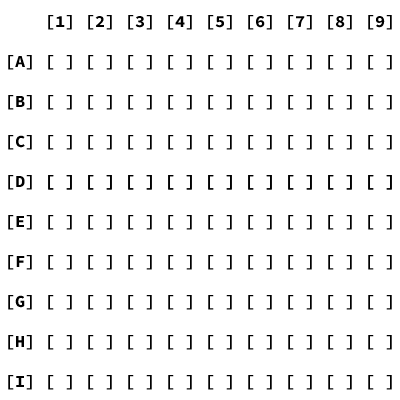
\includegraphics[width=0.5\textwidth]{Slike/PTP/PTP_Pocetak.png}
    \caption*{Slika 1}
    \label{fig:ptp_pocetak}
\end{figure}

Klijent unosi onoliko koordinata kolika je dužina broda ($1\times3$ zahteva 3 koordinate) u formatu {A,1 A, 2 A, 3} gde “A” predstavlja red, dok su brojevi 1, 2 i 3 kolone koje brod zauzima. Brod je potrebno iscrtati na tabeli tako što se polja koja zauzimaju popune znakom “o” i tabela se prikazuje klijentu (videti sliku 2). Kada klijent postavi sve brodove, serveru se prosleđuje tabela u formatu po želji. Server čuva tabele i čeka da oba igrača završe popunjavanje, a zatim ih obaveštava o početku sledeće faze igre.

\begin{figure}[H]
    \centering
    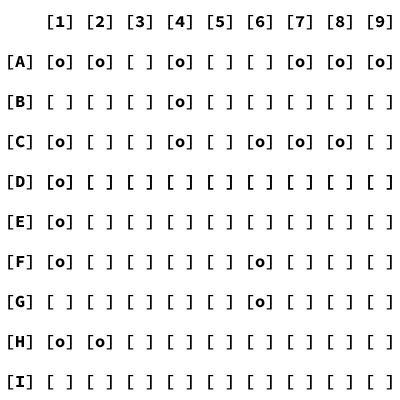
\includegraphics[width=0.5\textwidth]{Slike/PTP/PTP_Postavka.png}
    \caption*{Slika 2}
    \label{fig:ptp_postavka}
\end{figure}

\textbf{Faza II}

U ovoj fazi igrači napadaju i potapaju neprijateljske brodove. Klijent bira polje koje napada u formatu {E,6} i šalje poruku serveru. Server proverava da li se na tom polju nalazi neprijateljski brod ili ne, u zavisnosti od toga vraća “pogodak” ili “promašaj”. Igra traje dok igrač ne potopi sve brodove.

Pobednik je onaj koji potopi suigračeve brodove u manjem broju pokušaja. Klijenti igraju igru nezavisno jedan od drugog (ne postoje potezi). Nakon potapanja svih brodova klijent dobija poruku o svom skoru i obaveštenje da je završio igru.

Nakon kraja igre, protivnik može poslati poruku “status” kojom proverava da li je igra završena i ko je pobedio.

Napomena: sva komunikacija se dešava između klijenta i servera, igrači ne znaju ništa jedan o drugom, osim informacije ko je pobedio nakon poslate poruke „status“.

\begin{figure}[H]
    \centering
    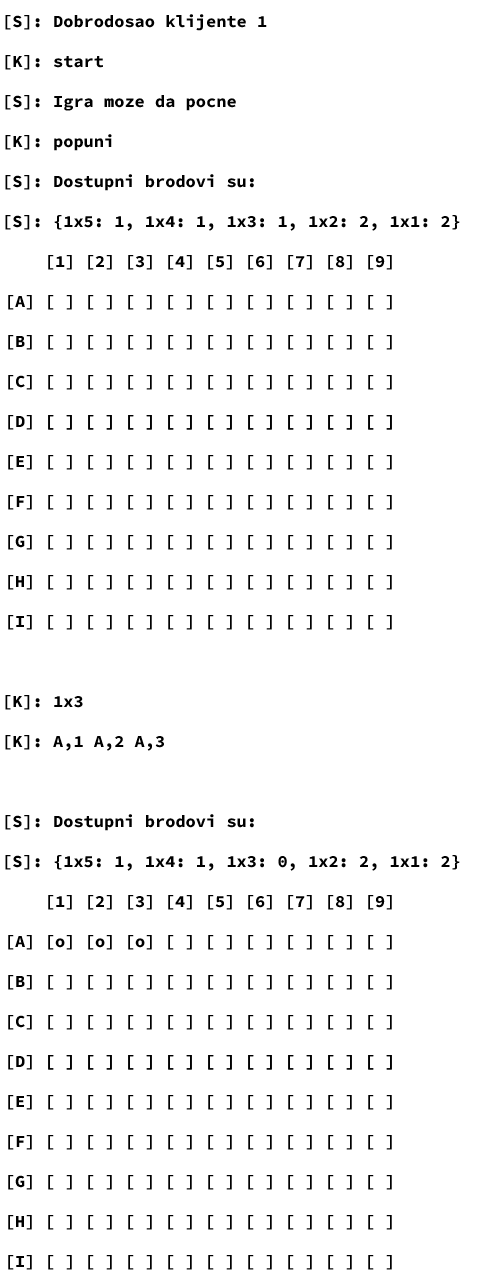
\includegraphics[width=0.5\textwidth]{Slike/PTP/PTP_Primer_komunikacije.png}
    \caption*{Primer postavke brodova}
    \label{fig:ptp_primer_postavke}
\end{figure}

Nakon raspodele svih brodova klijent šalje serveru metu i server mu vraća trenutan izgled table:

\begin{figure}[H]
    \centering
    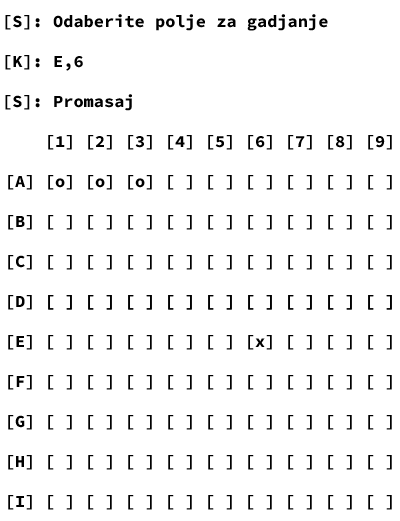
\includegraphics[width=0.5\textwidth]{Slike/PTP/PTP_Promasaj.png}
    \caption*{Primer promasaja}
    \label{fig:ptp_promasaj}
\end{figure}

\begin{figure}[H]
    \centering
    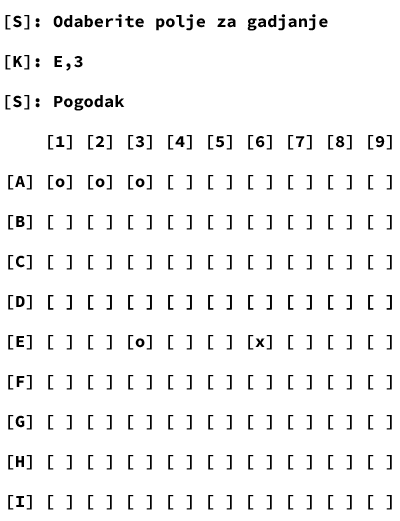
\includegraphics[width=0.5\textwidth]{Slike/PTP/PTP_Pogodak.png}
    \caption*{Primer pogodka}
    \label{fig:ptp_pogodak}
\end{figure}

Po završetku igre server obaveštava korisnika o kraju:

\begin{figure}[H]
    \centering
    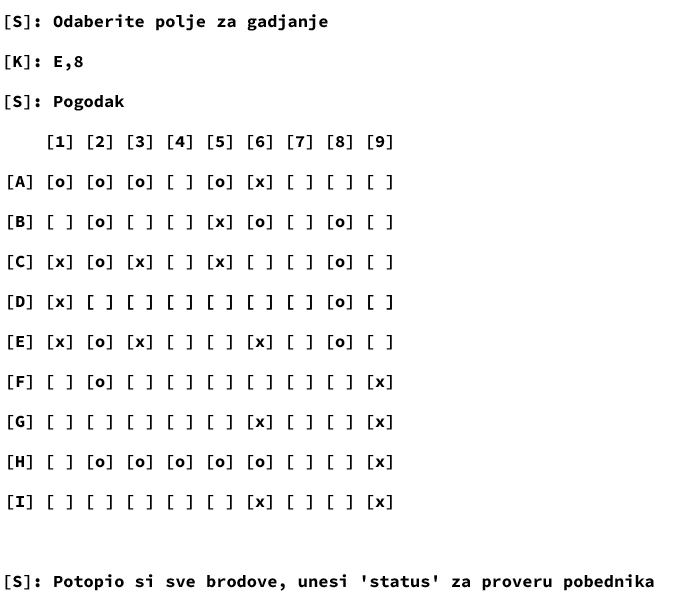
\includegraphics[width=0.8\textwidth]{Slike/PTP/PTP_Pobeda.png}
    \label{fig:ptp_pobeda}
\end{figure}

Provera statusa (moguće je da igra još uvek traje za drugog korisnika ili server ispisuje pobednika):

\begin{figure}[H]
    \centering
    
\includegraphics[width=0.5\textwidth]{Slike/PTP/PTP_Status.png}
    \label{fig:ptp_status}
\end{figure}